\section{Descripción general del entorno de pruebas}
En esta sección se presentan las parámetros adoptados para la configuración del entorno de
pruebas, que se encuentra dividido en : características de la población inicial, periodo y datos
climatológicos, parámetros de simulador del proceso evolutivo, y por ultimo, el hardware y sistema
operativo utilizados.

\subsection{Características de la población inicial}
La cantidad de puntos de control, utilizadas para las pruebas, fue seleccionada aleatoriamente,
teniendo en cuenta que debía ser un número múltiplo de 5 ya que existen 5 tipos de zonas
(ver \secref{subsec:cap4-zonificacion}). El número seleccionado fue 25 puntos de control, de ese
modo se cuenta con 5 puntos de control por cada tipo de zona. La cantidad de larvas que
corresponden a cada punto de control se generó forma aleatoria teniendo en cuenta que los límites
establecidos para cada tipo de zona (ver \tabref{tab:cap4-puntaje-zona}). En total contabilizaron
un total de 1.146 larvas para los 25 puntos de control.

\begin{table}[!htpb]
    \begin{minipage}{\textwidth}
    \centering
        \caption{\label{tab:valores-puntos-control} Conjunto de valores de los 25 puntos de control utilizados para las pruebas.}
        \begin{tabular}{c c c c}
            \hline\\
            Identificador& Cantidad$^a$& Longitud$^b$ & Latitud$^b$\\
            \hline
            \hline \\
            198 & 40 & -57,5865364153283 & -25,3133547921686 \\
            211 & 50 & -57,5855064470667 & -25,3227427549151 \\
            209 & 10 & -57,5789833147425 & -25,3173893777233 \\
            199 & 30 & -57,5882959444416 & -25,3158764238892 \\
            201 & 36 & -57,5926303942098 & -25,3218505418179 \\
            207 & 83 & -57,5898838121785 & -25,3235961699875 \\
            200 & 35 & -57,5909137804401 & -25,3193678272972 \\
            202 & 19 & -57,5948619921102 & -25,3249926544034 \\
            210 & 55 & -57,5814724047075 & -25,3201436810523 \\
            214 & 100 & -57,5870943148027 & -25,3187471407139 \\
            215 & 60 & -57,5834894258871 & -25,3160703933853 \\
            217 & 15 & -57,5887680132287 & -25,3207255681069 \\
            218 & 5 & -57,5934887010951 & -25,3273588828944 \\
            205 & 27 & -57,5879740793598 & -25,3313154239316 \\
            206 & 30 & -57,5893902857198 & -25,3292595903167 \\
            212 & 20 & -57,5830173571008 & -25,323402212545 \\
            213 & 65 & -57,5864076692956 & -25,3267382372734 \\
            223 & 71 & -57,5754213411705 & -25,3168462682653 \\
            219 & 16 & -57,5806570131676 & -25,3155660720482 \\
            216 & 49 & -57,5829315264117 & -25,3185919685716 \\
            203 & 90 & -57,591815002669 & -25,3297250651366 \\
            204 & 67 & -57,589840896834 & -25,3332936459521 \\
            220 & 45 & -57,5908997885579 & -25,3261169237658 \\
            221 & 53 & -57,5929597250812 & -25,3234791308407 \\
            222 & 75 & -57,5874236456741 & -25,3242937494949 \\
        \end{tabular}
        \footnotetext[1]{Cantidad de larvas correspondientes al punto de control.}
        \footnotetext[2]{Coordenadas geográficas correspondientes al punto de control.}
    \end{minipage}
\end{table}

En la \tabref{tab:valores-puntos-control}, se pueden apreciar los valores de los 25 puntos de
control utilizados. La distribución geográfica se realizó de forma aleatoria y no uniforme
en un área de total de $3,028 km^{2}$, que corresponde al área resultante de la unión de 2
barrios, Terminal e Hipódromo, de la ciudad de Asunción (\figref{fig:distribucion-puntos}).
Es importante aclarar que la selección de los barrios solo tiene relevancia, en la simulación,
para la obtención de datos climatológicos correspondientes para dicha región.

\begin{figure}[!htpb]
\centering
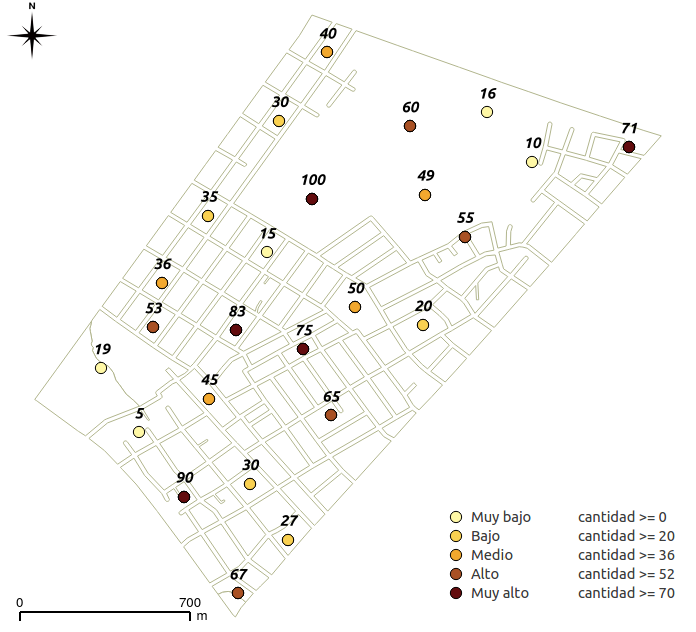
\includegraphics[width=0.9\textwidth]{./capitulo-6/graphics/extension-poblacion.png}
\caption{\label{fig:distribucion-puntos}Distribución geográfica de los 25 puntos de control.}
\end{figure}


\subsection{Periodo y datos climatológicos}
La mayoría de los estudios, que posteriormente fueron utilizados para las comparaciones, se basan
en someter a un grupo de individuos por un periodo de tiempo fijo utilizando una temperatura
constante. El mayor periodo observado fue de $46,83$ días en \cite{rueda1990temperature}, motivo
por el cual el tamaño del periodo fue establecido en 50 días.

En total se realizaron 10 iteraciones de 50 días cada una con las siguientes temperaturas :
15\textcelsius , 18\textcelsius , 20\textcelsius , 22\textcelsius , 24\textcelsius , 25\textcelsius
, 26\textcelsius , 27\textcelsius , 30\textcelsius , 34\textcelsius. De este modo se pueden simular
el proceso evolutivo de los individuos de la población a 10 temperaturas constantes.

\begin{figure}[!htpb]
\centering
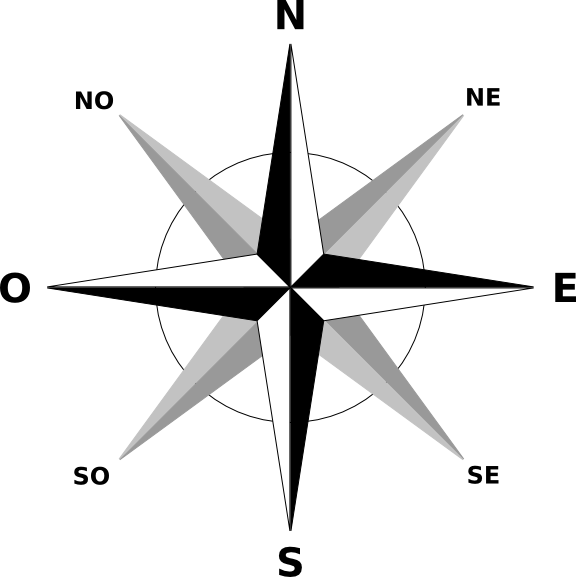
\includegraphics[width=0.5\textwidth]{./capitulo-6/graphics/rosa-de-vientos.png}
\caption{\label{fig:puntos-cardinales}Representación de los puntos cardinales.}
\end{figure}

La dirección al igual que la temperatura fue establecida como una constante para las pruebas, para
facilitar el análisis de la dispersión de los focos. La dirección del viento seleccionada fue la
suroeste (\figref{fig:puntos-cardinales}), que genera un ángulo que varía entre $202,5^{\circ}$ a
$247,5^{\circ}$.

\subsection{Parámetros de simulador del proceso evolutivo}
Los parámetros del simulador del proceso evolutivo, en su mayoría son calculados con datos
biológicos correspondientes al área de estudio. Obtener dichos datos requieren minuciosos estudios
de campo que escapan del alcance de este trabajo. Finalmente se optó por utilizar configuraciones
provenientes del material bibliográfico disponible que utilizado para el diseño y desarrollo del
modelo encargado de realizar la simulación de la ecología del vector.

El tamaño del radio, $r$, fue configurado en $200$ metros, para el cálculo de la densidad relativa
de larvas, $u(x,y)$ (ver \secref{subsec:cap4-zonificacion}). De este modo se incluirán todos los
puntos de control que se encuentren en un área de $125,663 \times 10^{3}$ $m^{2}$.

En cuanto a los sitios de reproducción, los parámetros $bs_{min}$ y $bs_{max}$ fueron
configurados según lo observado en \cite{otero2006stochastic, otero2008stochastic}, siendo $15$ y
$50$ los valores adoptados respectivamente.  El valor de $bs_{med}$ fue establecido, en $32,5$,
realizando un promedio entre $bs_{min}$ y $bs_{max}$.

En la \tabref{tab:coef-sharpe-demichele}, se pueden apreciar los coeficientes para el modelo
simplificado de Sharpe y DeMichele, con inhibición de altas temperaturas de Schoolfield (ver
\secref{subsec:cap4-tasas de desarrollo}) utilizados para calcular las tasas de desarrollo media
en $dias^{-1}$ fueron tomados de : \cite{rueda1990temperature} para el desarrollo larvario y el
desarrollo pupal, y de \cite{otero2006stochastic} para la eclosión de huevos, ciclo gonotrófico para hembras nulíperas y paridas.

\begin{table}[!htpb]
\begin{minipage}{\textwidth}
    \centering
    \caption{ \label{tab:coef-sharpe-demichele} Coeficientes para el modelo simplificado de Sharpe y DeMichele, con inhibición de altas temperaturas presentado por Schoolfield.}
    \begin{tabular}{p{6cm} c r r r r }
        \hline \\
        Ciclo de desarrollo    & $R(298K)$ & $\Delta H_{A}$ & $\Delta H_{H}$ & $\Delta T_{1/2}$  \\
        \hline
        \hline\\
        Eclosión de los huevos$^a$ & 0,24000 & 10798,00 &  100000,00  & 14184,000\\
        Desarrollo larvario$^b$    & 0,20429 & 36072,78 &   59147,51  &   301,560\\
        Desarrollo pupal$^b$       & 0,74423 & 19246,42 &    5954,35  &   302,687\\
        Ciclo gonotrófico (AN)$^c$ & 0,21600 & 15725,00 & 1756481,00  &   447,200\\
        Ciclo gonotrófico (AP)$^c$ & 0,37200 & 15725,00 & 1756481,00  &   447,200\\
    \end{tabular}
    \footnotetext[1]{Coeficientes tomados \cite{otero2006stochastic}.}
    \footnotetext[2]{Coeficientes tomados \cite{rueda1990temperature}.}
    \footnotetext[3]{Coeficientes, para el desarrollo del ciclo gonotrófico de hembras paridas (AP) y nulíparas (AN), tomados \cite{otero2006stochastic}.}
\end{minipage}
\end{table}

Las configuraciones adoptadas de
\cite{otero2006stochastic,otero2008stochastic,rueda1990temperature}, resultan válidas para las
pruebas, sin embargo pueden requerir una revisión general con el fin de realizar los ajustes
correspondientes teniendo en cuenta los datos ecológicos del área de estudio.

\subsection{Hardware y sistema operativo utilizados}
El hardware y el sistema operativo utilizados para realizar las pruebas, tienen las siguientes
características :
\begin{itemize}
\item Procesador : Intel Core i5-2430M
\item CPU : 2.40GHz × 4
\item Memoria : 8 GB
\item Sistema operativo : Ubuntu 13.10 x 64
\end{itemize}

